% Generated by paper/figures/src/fig_quality_time.py from the 46-prompt panel summaries
% (results/baseline46, results/budget, results/progressive46) and results/progressive46/sca_prog_vs_hrdit_dev_author_paired.csv.
\begin{figure}[t]
  \centering
  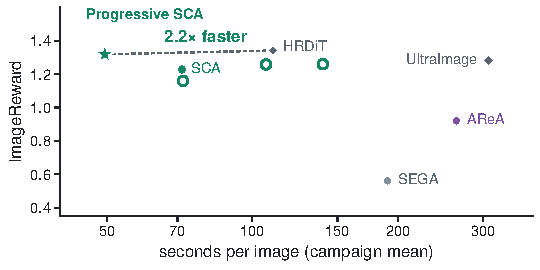
\includegraphics[width=\linewidth]{figures/quality_time.pdf}
  \caption{\textbf{Progressive \sca{} reaches HRDiT's ImageReward region in less than half its time, while more single-pass steps move \sca{} up more slowly.}
  Panel of 46 prompts at $4096^2$, seed~0; times are campaign means on shared GH200 nodes; diamonds mark multi-stage methods.
  Progressive minus HRDiT ImageReward: $-0.08$ $[-0.20,0.03]$ (95\% paired interval). Full attention, SigMa, and DyPE fall below the plotted range; Table~\ref{tab:panel46} lists all values.}
  \label{fig:quality_time}
\end{figure}
